\chapter{INDTRODUCTION}
%This chapter includes the following subtopics, namely: 
%(1) Rationale; 
%(2) Theoretical Framework;
% (3) Conceptual Framework/Paradigm; 
%(4) Statement of the problem; 
%(5) Hypothesis (Optional); 
%(6) Assumption (Optional); 
%(7) Scope and Delimitation;  and 
%(8) Importance of the study.

% =========================================================
%\section{Rationale}
% =========================================================
%This section have to explain: (a) the background of the study; (b) describe the problem situation considering global, national and local forces; (c) Justify the existence of the problem situation by citing statistical data and authoritative sources; and (d) Make a clinching statement that will relate the background to the proposed research problem.

% =========================================================
%\section{Theoretical Framework}
% =========================================================
%Discuss the theories and/or concepts, which are useful in conceptualizing the research.

% =========================================================
%\section{Conceptual Framework/Paradigm}
% =========================================================
%Identify and discuss the variables related to the problem, and present a schematic diagram of the paradigm of the research and discuss the relationship of the elements/variables therein.

% =========================================================
%\section{Statement of the Problem}
% =========================================================
%The general problem must be reflective of the title. It should be stated in such a way that it is not answerable by yes or no, not indicative of when and where. Rather, it should reflect between and among variables. Each sub-problem should cover mutually exclusive dimensions (no overlapping). The sub-problem should be arranged in logical order from actual to analytical following the flow in the research paradigm.

% =========================================================
%\section{Objective and Hypotheses}
% =========================================================
%First, explain the objective according the problem, then hypothesis. A hypothesis should be measurable/ desirable. It expresses expected relationship between two or more variables. It is based on the theory and/or empirical evidence. There are techniques available to measure or describe the variables. It is on a one to one correspondence with the specific problems of the study. A hypothesis in statistical form has the following characteristics: (a) it is used when the test of significance of relationships and difference of measures are involved; and (b) the level of significance if stated.

% =========================================================
%\section{Assumption}
% =========================================================
%An assumption should be based on the general and specific problems. It is stated in simple, brief, generally accepted statement.

% =========================================================
%\section{Scope and Delimitation}
% =========================================================
%Indicate the principal variables, locale, timeframe, and justification.

% =========================================================
%\section{Significance of the Study}
% =========================================================
%This section describes the contributions of the study as new knowledge, make findings more conclusive. It cites the usefulness of the study to the specific groups.


% =========================================================
\section{Latar belakang masalah}
% =========================================================
%2.     Pendahuluan (pada Bab 1)
%a.     Latar belakang masalah
%Berisi landasan permasalahan yang diperkuat dengan sitasi dari literature (Paper conference/paper jurnal/textbook 3 tahun terakhir). Permasalahan dapat diambil dari penelitian/pekerjaan sebelumnya dalam 3 tahun terakhir.
%Ringkasan Studi Pustaka/previous work/state of the art  tersebut terdiri dari 1-3 paragraf.
 %Berisi minimal 1.5 halaman. Pada alinea terakhir, nyatakan kaitan antara Tesis yang akan dibuat dengan penelitian/pekerjaan sebelumnya.
 
 
 %navigasi
 %Navigasi robot seluler dikategorikan ke dalam tugas2 berikut-:
- Membangkitkan model dunia dalam bentuk peta.
- Menghitung lintasan bebas tabrakan dari posisi awal ke posisi target. collision-free 
- Bergerak di sepanjang lintasan yang dihitung, menghindari tabrakan dengan rintangan. obstacles.
\cite{Rubio2019a}
 
 
 %Back ground should contain reasons of why phenomenon is chosen as the research topic; 
 %
 %Behavior based Arsitektur
 % Dalam banyak aplikasi robot, sering kali dibutuhkan reaksi yang cepat dari robot. Arsitektur behavior based control merupakan arsitektur robot yang cocok karena memiliki struktur behavior horizontal yang bekerja bersama secara paralel, bersamaan dan asinkronus (Brooks, 1986). 
 %Hexapod pertama yang digunakan dengan arsitektur behavior based ialah Genghis (Brooks, 1989) 
 
 %Pembelajaran RL
 %Selain arsitektur yang tepat, juga diperlukan mekanisme pembelajaran yang tepat pada robot untuk mengatasi hal – hal tak terduga. Reinforcement learning adalah metode unsupervised learning yang dapat belajar dari kritik/reward secara langsung (online) dari lingkungan, sehingga cocok untuk aplikasi robot. (Glorennec, 2000). 
 
 %Q-Learning
 %Ada berbagai metode untuk penyelesaian masalah reinforcement learning, salah satu yang paling populer ialah Q Learning Algorithm (Watkins, 1989). Kelebihan dari Q Learning ialah sifatnya yang off policy (dapat mengikuti policy apapun), algoritma yang sederhana, dan konvergen terhadap optimal policy (Perez, 2003). 
 
% The Q learning exhibited a long convergence time since it was affected by the generalization problem.
 
 
 Setiap tahunnya, lebih dari 2 (dua) juta ton plastik dibuang ke sungai dan akhirnya hanyut ke laut \cite{Othman2020}, sehingga sistem pembuangan sampah menjadi sektor yang cukup krusial \cite{Othman2020}\cite{Hossain2019}. Metode pengelolaan sampah secara manual menjadi metode yang sering digunakan untuk mengatasi krisis tersebut\cite{Khan2020}. Namun, terdapat beberapa masalah pada pengelolaan sampah secara manual, seperti keselamatan para tenaga kerja, tidak dapat menjaungkau daerah terpencil, tingginya biaya pengoprasian, dan lainya\cite{Khan2020}. Autonomous Robot menjadi solusi untuk mengatasi permasalahan tersebut, karena dapat mengurangi resiko kecelakaan, dapat menjangkau daerah terpencil, dan dapat melakukan pekerjaan secara berulang \cite{Khan2020, Bai2018}. Autonomous Robot telah banyak dikembangkan pada beberape penelitian, seperti: Robot pembersih dinding \cite{HouxiangZhang2006}, pembersih air\cite{Yuan2011}, dan pembersih lantai\cite{Bai2018, Kang2014, Palacin2004}. Berdasarkan pada sistem kerja Autonomous Robot, sistem pengelola sampah dapat dibuat secara otomatis\cite{Bai2018, Nagayo2019, Prasetyo2020}.
 
 Robot dapat bergerak secara mandiri berdasarkan lingkungannya seperti [5] dan bergerak manual berdasarkan perintah dari operator seperti [6]. Salah satu cara untuk mendapatkan informasi di sekitarnya adalah dengan menggunakan teknik pengindraan visual yang tidak membutuhkan banyak sensor [4], [8].
 Beberapa teknik navigasi mobile robot telah diaplikasikan, yaitu navigasi berbasis perilaku (behaviors), petunjuk daerah (landmark), dan berbasis penglihatan (vision) [4]. 
 
 
 %Dalam navigasi autonomos robot di lingkungan yang tidak terstruktur, sulit untuk mendapatkan model matematika yang tepat dari interaksi robot dengan lingkungannya. Karena keacakan yang melekat pada lingkungan  maka sulit untuk mendapatkan pengetahuan lingkungan yang lengkap \cite{Mustafa2019}. Kompleksitas tugas dapat diatasi dengan metode membagi dan memecah seluruh masalah menjadi subtugas yang lebih mudah dikelola. Pada Penelitian ini akan membuat arsitektur perilaku hierarkis karena dapat memisahkan tugas merancang perilaku (behavior) primitif atau mengadaptasi strategi yang diawasi yang berkoordinasi dengan perilaku belajar (learning behavior)  \cite{Hoffmann2003}.
 
 Karena model lingkungannya yang tidak terstruktur dan tidak diketahui, metode reinforcement learning dapat digunakan.  Meskipun banyak algortima Q-learning kontinyu diusulkan, namun hanya beberapa yang diterapkan pada aplikasi robot real untuk sistem navigasi autonomous mobile robot[20]. 
 
 %the gap of existing condition and the future condition;
 %who,where,when (auth,paper,year)
 %what (problem)
 %how(method)
 %

 %the problem identification; metode yang d usulkan dan kelemahan yg ada
 
 Pada Referensi \cite{Bai2018}, sebuah Autonomous Robot dibuat untuk mengambil sampah yang beroperasi di rumput. Robot mampu mendeteksi sampah secara otomatis dan akurat dengan menggunakan algoritma Deep Neural Network \cite{Kong2009}. Robot tersebut dilengkapi sensor ultrasonic\cite{Michael2008} dan sistem navigasi \cite{Wang2008}. Hasil pengujian menunjukan bahwa robot mampu mendeteksi sampah dengan akurasi 95\%. Pada makalah\cite{Arai2019}, Autonomous Robot dirancang menggunakan algoritma Convolutional Neural Network (CNN) untuk mendeteksi berbagai jenis sampah, seperti kaleng, botol plastik, dan kotak makan siang secara otomatis. Sistem robot mampu mendeteksi sampah secara outdoor. Berdasarkan data hasil pengujian\cite{Arai2019}, robot tersebut mampu mendeteksi sampah dengan tingkat kepresisian sebesar 95,6\% dan tingkat akurasi sebesar 96,8\%.
 
 Terispirasi dari makalah \cite{Bai2018} dan makalah\cite{Kong2009,Michael2008,Wang2008,Arai2019}, penelitian thesis ini bertujuan untuk merancang \textit{Autonomous Trash Collector System} (ATCS) menggunakan \textit{Deep Reinfocement Learning}  \cite{Mustafa2019}. Robot dilengkapi dengan sensor kamera dan sistem navigasi untuk mendeteksi posisi robot. Selain itu, ATCS juga dilengkapi sistem kendali \textit{Adaptive Neuro-Fuzzy Inference System} (ANFIS) sebagai sistem kendali pada motor\cite{Saputra2019}. Penelitian ini diharapkan dapat membantu mengatasi masalah pengelolaan sampah yang kebanyakan masih dikelola secara manual.
  %bahas referensi utama,


%NEURO-FUZZY DEEP Q-LEARNING


possibility that the phenomenon will give new concepts as a result; 
%Pada penelitian ini terdapat beberapa behavior yang digunakan dalam aplikasi robot soccer, diantaranya wandering (berkeliling), search target (bola), dan go to goal (gawang). Behavior dengan tujuan berbeda dapat menimbulkan konflik yang tidak dapat diselesaikan. Oleh karena itu, dibutuhkan suatu formulasi mekanisme koordinasi yang efektif dari beberapa aktifitas robot .

%====================================
%Pada penelitian ini akan dirancang hexapod robot dengan arsitektur behavior based. Kemudian juga akan ditambahkan Q learning sebagai mekanisme pembelajaran robot. Robot akan melakukan navigasi otonom untuk menghindari halangan dan menemukan target berupa sumber cahaya.


%Pada penelitian ini terdapat beberapabehavior yang digunakan dalam aplikasi robot soccer, diantaranya wandering (berkeliling), search target (bola), dan go to goal (gawang). Behavior dengan tujuan berbeda dapat menimbulkan konflik yang tidak dapat diselesaikan. Oleh karena itu, dibutuhkan suatu formulasi mekanisme koordinasi yang efektif dari beberapa aktifitas robot .

%Pada penelitian ini akan dirancang robot multiplatform iSRo II dengan arsitektur behavior based control. Algoritma FQL hanya diterapkan pada dua prilaku yaitu menghindari rintangan, dan mencapai target.



% =========================================================
\section{Rumusan masalah}
% =========================================================
%Berisi urutan permasalahan yang dihadapi untuk menyelesaikan penelitian, dalam 1 kalimat. Buat dalam bentuk point rumusan masalah dan berisi minimal ½  halaman.
%Problem identification, Objective, Relation between problems and objective
%The relation between the previous research or the existing condition and the reference, The relation between problem definition and research variable.
%The objective answerS the problem AND solves the problems, the hypothesis is built based on the objecctives and the problems. The objective is specific
\begin{itemize}
	\item Sensor kamera CNN pada pengolahan Digital Image Processing
	\item Navigas autonomous robot pada lingkungan dinamik
	\item Algoritma Q-Learning dengan Neuro Fuzzy
\end{itemize} 


% =========================================================
\section{Tujuan}
% =========================================================
%Berisi tujuan penelitian yang ditulis dalam bentuk satu kalimat dan dirinci langkah-langkah nya dalam bentuk point tujuan dan berisi minimal ½ halaman.
%Objective and Hypotheses (Tujuan dan Hipotesa)
%This section should contain objective research direction (sharp and measurable) and the hypotheses (The explanation of method, concept which will be used to solve the problem as well as the reason why they will be used in the research; the explanation about the difference between method, concept, and theorem which will be used and the method, concept method, concept which were used previously ).
\begin{itemize}
	\item Q-Learning, obstacle avoidance dan mobile robot
	\item 
\end{itemize}
% =========================================================
%\section{Hipotesis}
% =========================================================
%Berisi prediksi hasil dan dasar prediksi yang digunakan berdasarkan referensi hasil pekerjaan/penelitian sebelumnya. Sertakan referensi yang disitasi untuk memprediksi hasil. Hipotesis Berisi minimal ½ halaman.
   
    %Deteksi presisi tinggi dapat membantu robot menyelesaikan tugas dengan lebih akurat, andal, dan stabil. Performa SSD dan R-CNN yang Lebih Cepat dalam akurasi jauh lebih rendah daripada jaringan YOLOv3. Kerangka dasar SSD dan Faster R-CNN adalah VGG16, VGG19, dan Res101, sedangkan jaringan dasar YOLOv3 adalah Darknet-53 \cite{Li2020}.
    
   %Pengontrol ANFIS penghindaran rintangan diaktifkan untuk menghindari rintangan. Setelah setiap titik penghindaran, robot beralih ke target mencapai pengontrol ANFIS. Dalam kedua skenario yang dipertimbangkan, mobile robot mampu menghindari rintangan dengan aman dan mencapai target dengan jalur yang dihasilkan secara online yang layak dan mulus antara titik awal dan titik target. \cite{Al-mayyahi2014}.
    
 %Dari hasil simulasi terlihat bahwa waktu pelatihan pada sistem RL berbasis     Dynamic Evolving Fuzzy-Neural Network (DENFIS) lebih besar dibandingkan dengan sistem RL berbasis Q-learning dinamis fuzzy. Fitur ini dicapai tanpa kehilangan kinerja \cite{Shah2014}.
    
\section{Scope of Work}
%Scope of work  concerns about the knowledge (reference), (facility, usability and user  OPTIONAL)

\begin{enumerate}
	\item Lokasi pengujian dilakukan di ruangan tertutup dan menggunakan lingkungan buatan.
	\item terdapat obyek, target sampah dan obstacle untuk dihindari yang disimpan secara acak
	%\item sampah yang dideteksi terdiri dari lima jenis
	%\item Menggunakan kamera webcam sebagai penangkap citra atau gambar pada Image Processing.
	\item Jenis robot yang digunakan adalah non platform mobile robot yang dirancang sendiri.
	\item Pada perancangan sistem tidak dilakukan perhitungan terhadap parameter motor dc seperti gaya gesek dan inersia.
	\item Sistem kendali gerak hanya mengontrol kecepatan dan arah putar motor dc pada mobile robot.
	\item Sistem navigasi mobile robot ini beroperasi pada lintasan yang datar.
\end{enumerate}


\section{Research Method}
% =========================================================
%Berisi penjelasan singkat tentang metode/formula/skema/algoritma utama (1-2metoda) yang  akan digunakan/diusulkan dalam penelitian, berdasarkan referensi utama yang akan dijadikan acuan.

%- digital image processing (CNN/) \\

%CNN dengan learned-features (fitur hasil-pembelajaran) yang dihasilkan dapat digunakan untuk menyelesaikan permasalahan-permasalahan yang ada pada proses pengenalan objek dan pemulihan citra, misalnya pada metode pengenalan dan kategorisasi tempat.
%”The development of a robot control architecture for an AUV-able to achieve simple tasks and exhibit real-time learning capabil- ities”

Behavior-based control layer. Design of a behavior-based control system which will be contained in the overall control architecture with the purpose of accomplishing simple tasks. A task is intended as one of the phases in which a mission can be divided. It is assumed that the sequential achievement of a set of tasks entails the achievement of the mission. The behavior-based control system must assure the safety of the robot while demonstrating a high control performance.

Reinforcement Learning-based behaviors. Integration of a reinforcem- ent learning algorithm in the control architecture. This learning theory will be applied to the acquisition of the internal structure of a robot behavior. The purpose of using Reinforcement Learning is to reduce the required human work in the development of a new robot behavior. Instead of implementing the action-decision rules, the designer need only to define the goal of the behavior.

Experimentation with an AUV. Evaluation of the proposed control and learning systems with real experiments using an Autonomous Under- water Vehicle. The feasibility and limitations of these approaches must be experimentally tested with the available systems and resources.


Algoritma Neuro Fuzzy Q Learning pada sistem inferensi neuro-fuzzy adaptif telah diterapkan untuk mengontrol kecepatan sudut roda kendaraan darat otonom. Kecepatan ini memandu kendaraan dengan aman untuk mencapai tujuan dalam lingkungan statis tanpa bertabrakan dengan rintangan yang ada di jalan. Sistem yang diusulkan menggunakan empat pengontrol ANFIS. Pertama, dua pengontrol untuk pencapaian target yang memastikan kendaraan mencapai titik tujuannya; Kedua, dua pengontrol untuk memandu kendaraan untuk menghindari tabrakan dengan rintangan. Dalam empat pengontrol ini, kecepatan sudut kanan dan kiri akan menurunkan arah kendaraan selama navigasi \cite{Al-mayyahi2014}.
% =========================================================
      

%NFQ-Learning daiagram blok
%



\section{Metodologi}
% =========================================================
%Berisi urutan langkah – langkah untuk menyelesaikan penelitian beserta teknik/metoda disetiap langkah. Buat dalam bentuk diagram blok dan deskripsikan setiap langkah tersebut. Berisi minimal 1 halaman.

%This section contains reference tracing, requirement identification, design process, implementation process, experiment design and plan, analysis method berisi minimal 1 halaman.
%This section should contain the following procedure
%1.	Reference tracing
%2.	Requirement identification
%3.	Design process
%4.	Implementation process 
%5.	Experiment design and plan (including data collection process)
%6.	Analysis/Evaluation method which will be used for analyzing the experiment result
Adapun tahapan pada penelitian adalah sebagai berikut:

\begin{figure}[H]
	\centering
	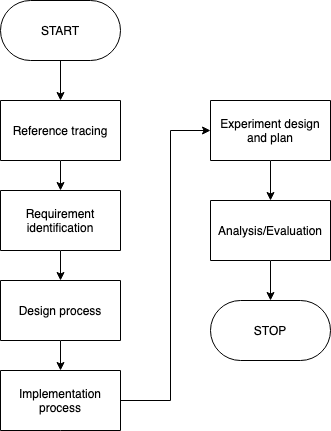
\includegraphics[width=0.7\linewidth]{figure/Metode-Penelitian-flow.png}
	\caption[Metode Penelitian]{}
	\label{fig:metode-penelitian-flow}
\end{figure}


%a. Study Literature
%In this step, this thesis studies the theories needed to design Early Warning System from textbooks, journals, conference papers, thesis or dissertation books, and interview with tea researcher. In this stage, design thinking is also done to  nd out the problems and what are the user needs.
%b. Requirements Analysis
%n this stage, requirements analysis is carried out in accordance with the requirements of the system to be built included requirements of hardware and software (determine tools, materials, and speci cation).
%c. System Design
%A System design and manufacturing device will be done in this stage. System will be designed generally from physical layer to application layer. Arti cial Intelligence algorithm will be implement in this stage too.
%d. testing
%e. Evaluation
%Improve the system according to the feedback that has been obtained. The purpose of this stage is to create a system that is in accordance with user needs.
% f. Final Test, Result and Analysis
%Implementation and testing of the Early Warning and Monitoring System. In this stage, system performance analysis will be carried out.
%g. Reporting
%Writing the  nal report of research and journal publications.

\subsection{Reference tracing}
Studi literatur tentang :
Behavior based Robotic, Navigasi Visual, Reinforcement Learning, Q-learning, Neuro Fuzzy Q-learning, metode Simulasi Mobil Robot.

\subsection{Requirement identification}

Pada tahap ini dilakukan analisis yang mencangkup kebutuhan untuk melakukan penelitian, kebutuhan yang dianalisis dibagi menjadi analisa data dan juga analisa kebutuhan sistem. Analisis dilakukan agar sistem yang dibangun dapat berjalan sesuai dengan rancangan yang sebelumya sudah ditentukan.

\subsection{Design process}
Melakukan desain robot dari segi mekanika, elektronika dan algoritma agar robot bisa berjalan sesuai tujuan.

\subsection{Implementation process }
Pada tahap ini merupakan tahap untuk perancangan, yaitu bertujuan untuk mengimplementasikan navigasi, target tracking dan localization pada mobile robot menggunakan sensor kamera. Serta melakukan trial error pada pada pergerakan robot.

\subsection{Experiment design and plan}
Selanjutnya dilakukan pengujian terhadap mobile robot dan program deteksi posisi obyek. Pengujian dilakukan dalam beberapa aspek, yaitu: sudut cakupan mobile robot, deteksi posisi obyek pada gambar yang ditangkap oleh mobile robot, jarak jangkauan deteksi posisi obyek pada gambar yang ditangkap oleh robotic vision system, deteksi posisi obyek di lapangan, kecepatan program deteksi posisi obyek.

\subsection{Analysis/Evaluation}
%edit:
Berdasarkan pengujian yang dilakukan untuk selanjutnya dianalisis mengenai keberhasilan pembuatan robotic  system berdasarkan pengujian sudut cakupan mobile robot. Sedangkan keberhasilan program deteksi posisi obyek (obstacle dan Sampah) berdasarkan pengujian deteksi posisi obyek pada gambar yang ditangkap oleh mobile robot, pengujian jarak jangkauan deteksi posisi obyek pada gambar yang ditangkap oleh mobile robot, pengujian deteksi posisi obyek di lapangan, pengujian kecepatan program deteksi posisi obyek.

\section{Schedule}

%The schedule match the research method and feasible to be realized
%Timetable/Schedule (jadwal pelaksanaan)
%Activity	1	2	3	4	5	..	..
%Reference tracing							
%Requirement identification							
%Design process							
%Implementation process							
%Experiment design and plan							
%Analysis/Evaluation							

Penelitian ini direncanakan akan diselesaikan dalam tempo empat bulan. Rencana tersebut dijabarkan dalam tabel sebagai berikut:

%Pembuatan Usulan Penelitian

%Kajian Pustaka

%Desain algoritma kontrol

%Simulasi Robot

%Pengujian pada robot aktual

%Pembuatan laporan

%Seminar Hasil

\begin{figure}[H]
	\centering
	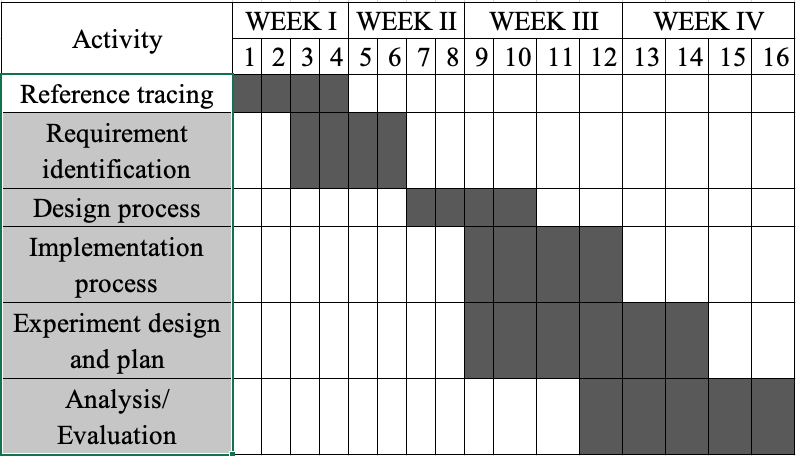
\includegraphics[width=0.9\linewidth]{figure/Chart-ThesisQ.png}
	\caption{Usulan Penelitian}
	\label{fig:chart-thesisq}
\end{figure}


In order to develop an autonomous robot, a control architecture must be included in the robot control system. The control architecture has the goal of accomplishing a mission which can be divided into a set of sequential tasks.  Behavior-based control architectures as a methodology to implement this kind of controllers. Its high interaction with the environment, as well as its fast execution and reactivity, are the keys to its success in controlling autonomous robots. This chapter also compared some classic approaches by testing their performance in a simulated task with an Autonomous Underwater Vehicle. The main attention was given to the coordination methodology. Competitive coordinators assured the robustness of the controller, whereas cooperative coordinators determined the performance of the final robot trajectory. Chapter 3 proposed the structure of a control architecture for an autonomous robot. Two main layers are found in this schema; the deliberative layer which divides the robot mission into a set of tasks, and the behavior-based layer which is in charge of accomplishing these tasks. This chapter and the thesis centered only on the behavior-based. layer. A behavior coordination approach was proposed. The main feature is its hybrid coordination of behaviors, between competitive and cooperative approaches. The approach was tested with the simulated task as well.


The second part of the thesis centered on the implementation of the robot
behaviors. It proposed the use of a learning algorithm to learn the internal mapping between the environment state and the robot actions. Chapter 4 presented Reinforcement Learning as a suitable learning theory for robot learning. Its online applicability and the non-requirement of any previous information about the environment are the most important advantages. In addition, the Q learning algorithm was presented, which is specially ade- quate for its capability in off-policy learning. The most important drawback is the generalization problem. Reinforcement Learning algorithms are based on discrete representations of the state and action spaces. When these algorithms are applied to continuous variables, as most robotics applications require, the discretization of the variables causes an enormous number of states and a long learning time. The generalization makes the application of Reinforcement Learning in robotics impractical. However, several techniques were presented which attempt to solve this problem. Chapter 5 proposed a Reinforcement Learning algorithm designed to be applied to robotics. The goal of the SONQL algorithm is to learn robot behaviors. It is based on the Q learning algorithm and solves the generalization problem by using a Neural Network and a database of the most representative learning samples.
The


%Contributions
%This thesis has accomplished the proposed goal which is the development of a robot control architecture for an AUV able to achieve simple tasks and exhibit real-time learning capabilities. In the development of this goal, some research contributions were achieved. Hereafter these contributions are listed:

%Online learning of robot behaviors . The most important contribution has been the online learning of robot behaviors. The use of Reinforce- ment Learning in robotics is very common nowadays. However, there are not many approaches which perform an online learning. It is, there- fore, an important contribution to demonstrate the feasibility of the SONQL in a real-time task, specially in a complex domain such as un- derwater robotics. The algorithm proved able to learn the state/action mapping of one DOF in less than 400 iterations, which was less than two minutes. Although the best parameters were used and the exper- iments were designed in detail, these results point out the important role learning algorithms will have in future robotics applications.

%SONQL as a continuous state RL algorithm . The second contribu- tion is also related to the SONQL algorithm. This algorithm demon- strated a high generalization capability in the ”mountain-car” bench- mark. The combination of the Neural Network and the learning sam- ples database resulted in an algorithm able to face the generalization problem. The Neural Network offered a high function approximation capability, and the database guaranteed its stability by avoiding the interference problem. To the best of the author’s knowledge, similar approaches have not been found in the literature and, therefore, the SONQL represents a contribution in the Reinforcement Learning field. However, it must be noted that, although the action space is contin- uous in the Neural Network, the search of greedy actions requires a discretization of this space. Therefore, the SONQL must be considered only as an algorithm to solve the generalization problem in the state space.

%Methodologies for Generalizing . The generalization problem in Rein- forcement Learning was treated in detail. The most important method- ologies currently being applied were described. This study was not considered as an exhaustive survey but a general overview of the most used techniques.

%Development of a behavior-based control system . Another contri- bution was the development of the behavior-based control layer, and in particular, the hybrid coordination methodology. The main features of the coordination system are its simplicity and robustness which assure the safety of the vehicle. In addition, the cooperation between behaviors improves the final robot trajectory. The behavior-based control layer demonstrated as being an efficient tool in the implementation of a set of behaviors and the obtained results were highly satisfactorily.

%Behavior-based control architectures . Four classic Behavior-based con- trol architectures were presented, tested and compared. These archi- tectures represent the most important principles in this field. There- fore, this study offers an exemplified introduction to Behavior-based Robotics. The testing of the architectures in a simulated environment also led to the identification of the dynamics model of ATCR robots.

%tdk d pakai.  ///  jd bahan paper?
%Development of a localization system . A localization system for un- derwater robots in structured environments was proposed. The system is able to estimate the position and orientation in three degrees of free- dom and also the velocity. The localization is based on a coded pattern and a computer vision system. The high accuracy of the estimations and the real-time execution of the algorithm are the main features. The localization system has been one of the most important factors for the success of the presented experiments.